\chapter{Usage Scenarios}
\thispagestyle{pagestyle}

In this chapter, I will present several scenarios showcasing Pie's usage, demonstrating how Pie can replace a code editor for daily activities. Each use case will be supported by screenshots and detailed paragraphs highlighting the application's interface.

\section{Writing HTML code and rendering it}

Code editing is the most frequently used functionality in Pie. The Scintilla editor is visible from the start of the application, and code support becomes available once the user saves the editor's content in a file.

I will open an HTML page with Pie, downloaded from a template found online. This will demonstrate how Pie's syntax highlighting works after identifying the file extension. Next, I will right-click inside the editor and select "Render HTML". The rendering task can also be initiated from the "Run" component in the docked menu strip.

\begin{figure}[h]
\centering
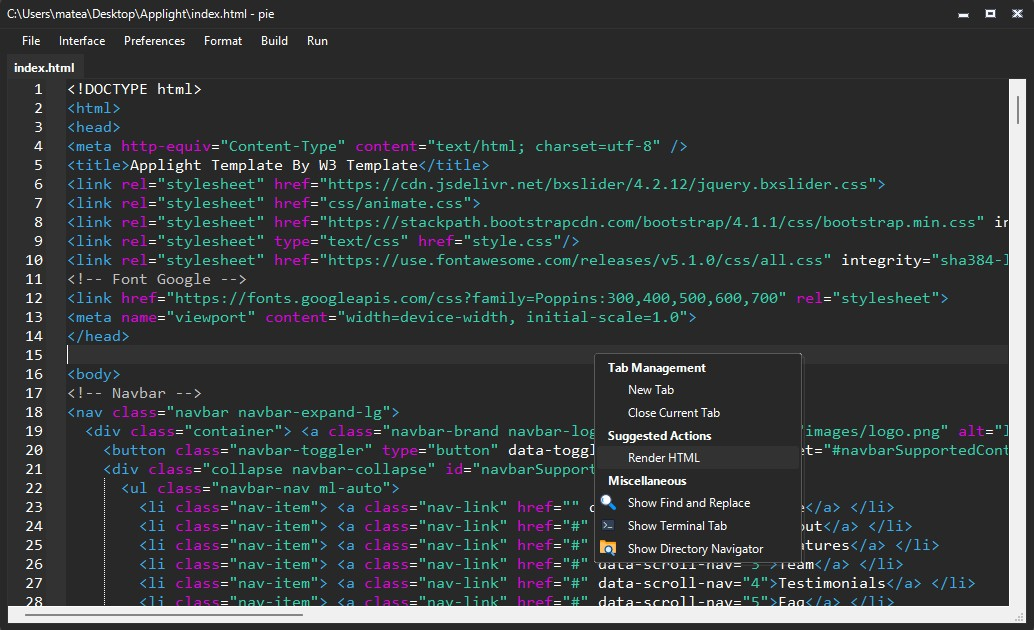
\includegraphics[width=0.7\textwidth]{images/render-context-menu.jpg}
\caption{Syntax highlighting for HTML code in Pie}
\label{fig:fig2,1.}
\end{figure}

Pie will open a new tab with the rendered HTML page. I can now switch between the two tabs and continue editing the source code. If any modifications are made, I can simply go to the second tab and refresh the page using the right-click context menu.

\begin{figure}[h]
\centering
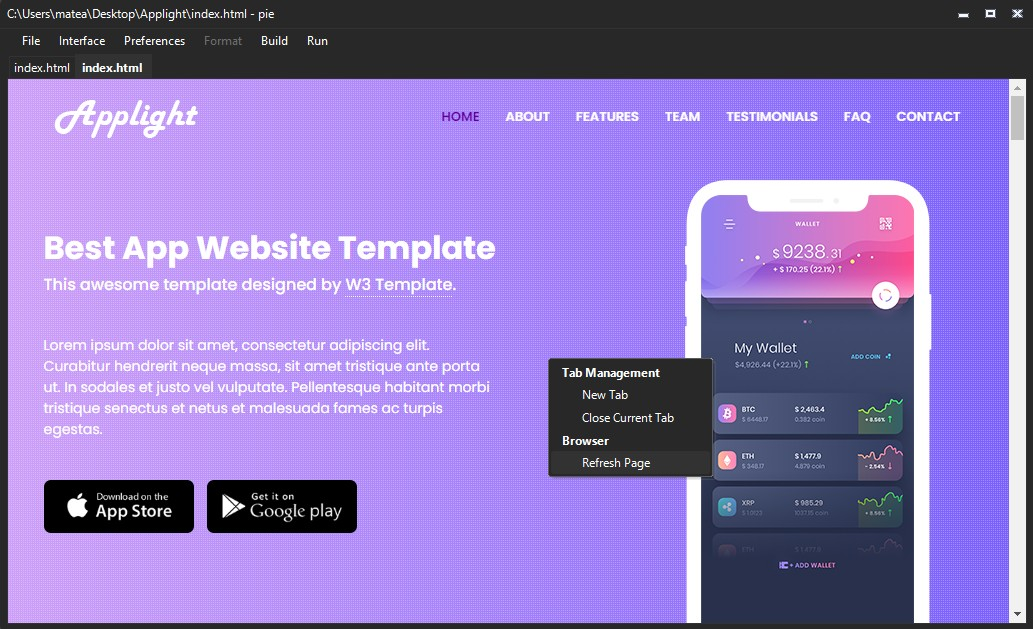
\includegraphics[width=0.7\textwidth]{images/render-output.jpg}
\caption{A rendered HTML page being displayed by Pie}
\label{fig:fig2,1.}
\end{figure}

\section{Running a Python script}

I will continue demonstrating the functionalities of the code editor by running a simple Python script that receives user input. This will highlight the capabilities of the ConEmu terminal and its seamless integration with Windows Forms applications.

\begin{figure}[H]
\centering
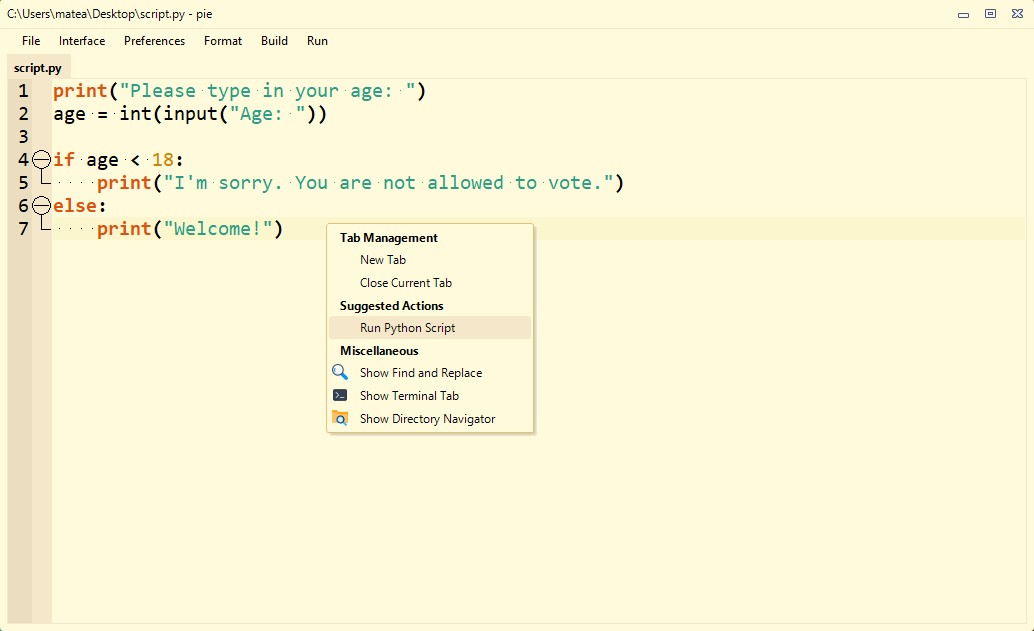
\includegraphics[width=0.7\textwidth]{images/python.jpg}
\caption{Python syntax highlighting in Pie}
\label{fig:fig2,1.}
\end{figure}

I can now click on the "Run Python Script" button in the "Suggested actions" category of the context menu. Pie dynamically adjusts context menu items based on factors such as the file extension, the number of custom build commands added, or the number of database connections stored internally. In this case, the script could also be launched from the "Run" button mentioned earlier.

\begin{figure}[H]
\centering
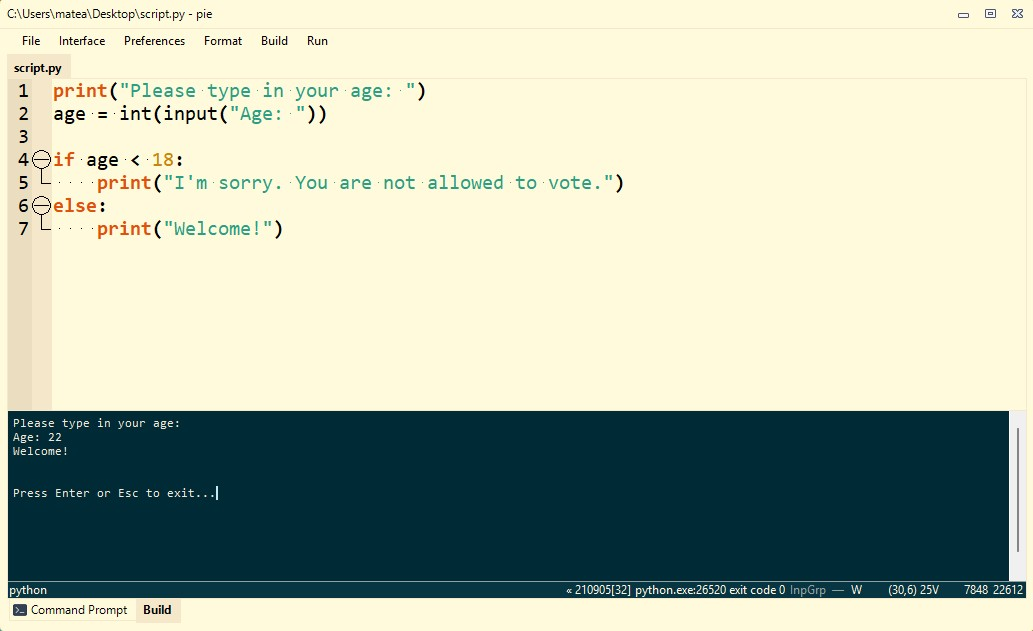
\includegraphics[width=0.9\textwidth]{images/python-output.jpg}
\caption{Output of a Python script being displayed in a ConEmu terminal instance}
\label{fig:fig2,1.}
\end{figure}

\section{Managing custom build commands}

In addition to predefined Build \& Run options (such as "Render HTML" and "Run Python Script"), users can also add their own build commands from the "Preferences" menu. Selecting "Build Commands" will open a list of current commands and allow for their management. Double-clicking on an existing build command lets the user edit it. I have edited the "My custom build command" entry, which now runs the \texttt{javac} command to compile a Java source.

\begin{figure}[H]
\centering
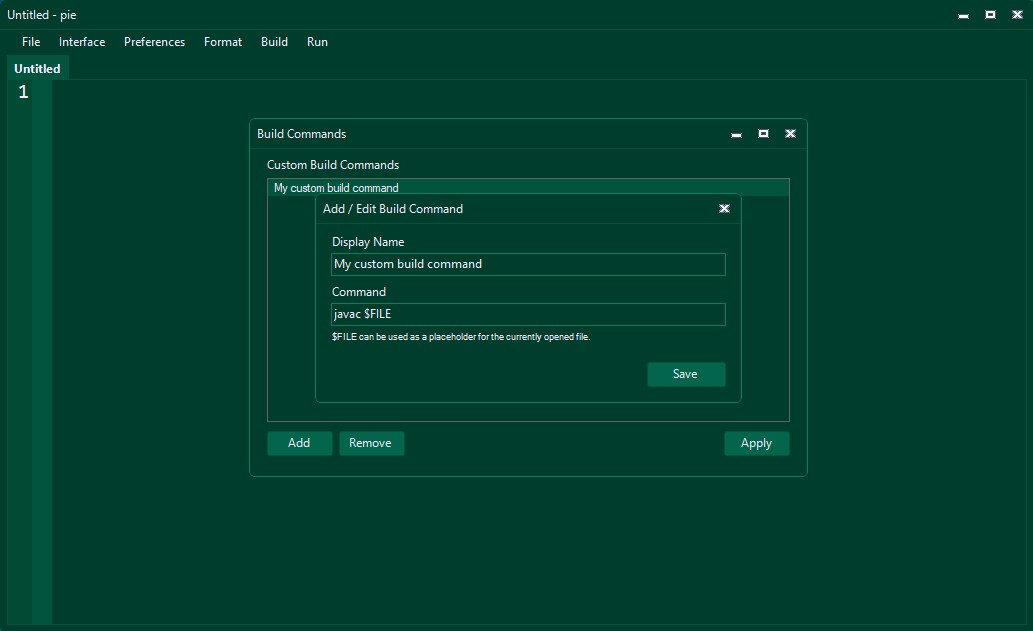
\includegraphics[width=0.6\textwidth]{images/editing-build-command.jpg}
\caption{Editing an existent build command}
\label{fig:fig2,1.}
\end{figure}

Custom build commands will be displayed in the "Run" menu component, regardless of the file's extension. The only requirement is to have a file open in the selected tab.

\begin{figure}[h]
\centering
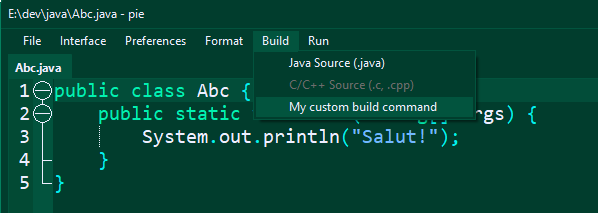
\includegraphics[width=0.6\textwidth]{images/running-build-command.png}
\caption{Pie displaying a custom build command in the "Run" menu item}
\label{fig:fig2,1.}
\end{figure}

\section{Navigating between directories}

The context menu in the \texttt{CODE} tabs offers a "Show Directory Navigator" option. By clicking on it, a panel will appear, listing all the directories and files from a specific folder. This panel can also be activated by pressing the Ctrl + G key combination.

\begin{figure}[H]
\centering
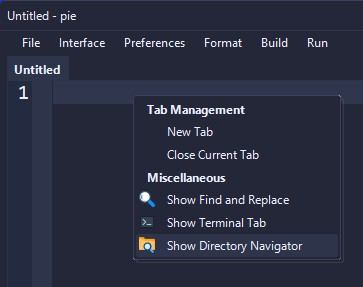
\includegraphics[width=0.5\textwidth]{images/directory-navigator.jpg}
\caption{Toggling the Directory Navigator from Pie's context menu}
\label{fig:fig2,1.}
\end{figure}

Double-clicking on a directory will display the items within that directory, while double-clicking on a file will open the file in a new \texttt{CODE} tab.

\begin{figure}[H]
\centering
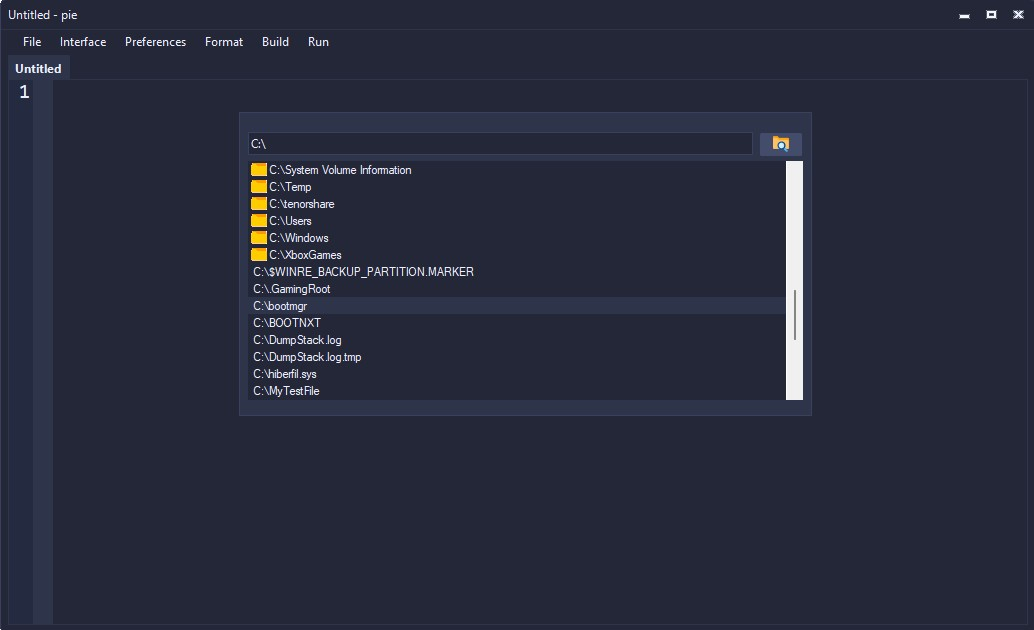
\includegraphics[width=0.7\textwidth]{images/directory-navigator-C.jpg}
\caption{Pie's Directory Navigator displaying the contents of drive C:\textbackslash}
\label{fig:fig2,1.}
\end{figure}

\section{Exploring Git repositories}

Users can access an advanced version control system interface by clicking on "Show Git Tab" under the "Interface" menu item.

\begin{figure}[H]
\centering
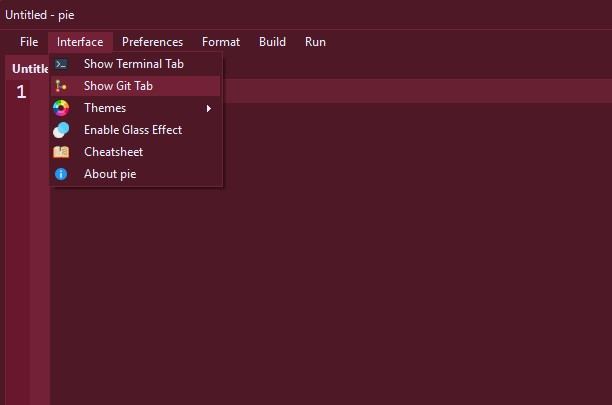
\includegraphics[width=0.7\textwidth]{images/show-git-tab.jpg}
\caption{Accessing the Git tab from the "Interface" menu}
\label{fig:fig2,1.}
\end{figure}

The displayed Git tab allows users to perform multiple actions, such as opening a local repository, cloning a remote one, or commiting changes. By clicking on the "Open local repo" button (as shown in the figure below), users can select a local repository to open. Once opened, all the files in the repository, along with their status, will be listed.

\begin{figure}[H]
\centering
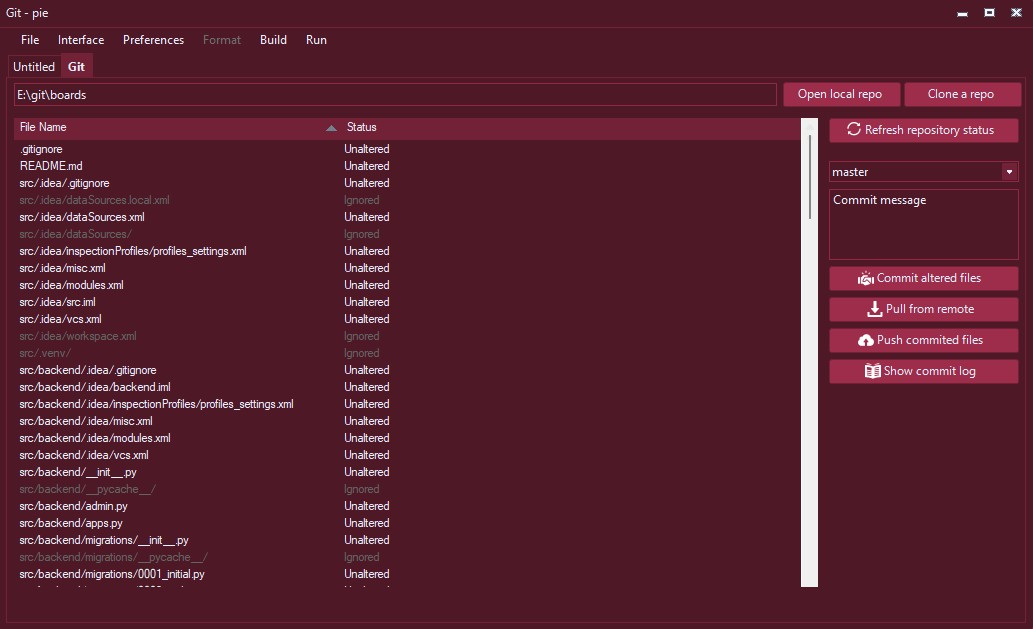
\includegraphics[width=0.7\textwidth]{images/git-tab.jpg}
\caption{Pie's Git tab, displaying an open repository}
\label{fig:fig2,1.}
\end{figure}

Developers can also sort files based on their status, making it easy to see which files are ignored and which not. Double-clicking one or more files in the ObjectListView control will open them in separate tabs, allowing the developer to edit them. I will open the \texttt{README.md} file, edit it, and then click on the "Refresh repository status" button to check if Pie has registered my changes.

\begin{lstlisting}[caption={Content of the README.md file before edit}]
# test repository
\end{lstlisting}

\begin{lstlisting}[language=json, caption={Content of the README.md file after edit}]
# test repository
This is a simple edit, in order to show Pie's advanced Git functionalities
\end{lstlisting}

\begin{figure}[H]
\centering
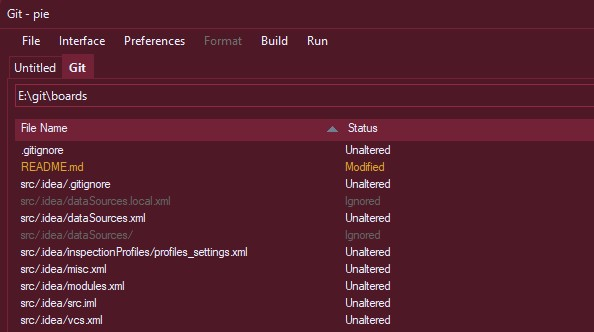
\includegraphics[width=0.7\textwidth]{images/pie-readme-git.jpg}
\caption{README.md being identified as modified in Pie's Git interface}
\label{fig:fig2,1.}
\end{figure}

Clicking "Commit altered files" will automatically stage the \texttt{README.md} file and then commit it with the message entered in the textbox above the commit button.

\section{Formatting text: sorting lines and removing whitespaces}

The "Format" menu item offers a consolidated list of the most commonly used formatting techniques, such as replacing whitespaces with commas, capitalizing every word, sorting lines in ascending or descending order, and trimming every line. Users can also type keywords in the "Search" text box, and the list of algorithms will update in real time. They can search based on the technique's name, category, or description.

\begin{figure}[H]
\centering
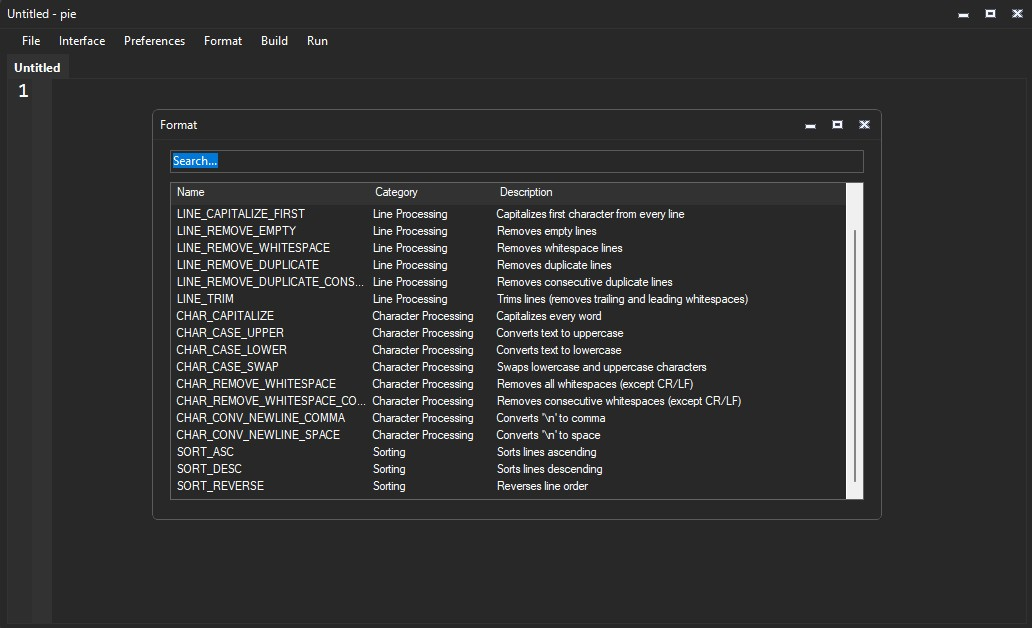
\includegraphics[width=0.7\textwidth]{images/format-menu.jpg}
\caption{Pie's Format menu}
\label{fig:fig2,1.}
\end{figure}

I will type a list of names inside my code editor, each name delimited by a newline (\textbackslash n).

\begin{lstlisting}[caption={List of random names that is going to be processed by Pie's formatting algorithms}]
John
Josh
Anna
Mark
Mario
Anthony
Jackson
Maria
Clarence
Stephan
\end{lstlisting}

I will now select the \texttt{SORT\_ASC} option from the "Format" menu by double-clicking on it. The result, directly written in the Scintilla editor, is displayed in the code snippet below:

\begin{lstlisting}[caption={Output after sorting lines ascending}]
Anna
Anthony
Clarence
Jackson
John
Josh
Maria
Mario
Mark
Stephan
\end{lstlisting}

I might want to initialize a list in Python with these names. For this, I need the names to be delimited by commas instead of newline characters. While doing this manually for 10 names is feasible, in production, such a list may contain hundreds or even thousands of entries. Relying on an online formatter may not be an option due to confidentiality purposes, but Pie can handle this easily in a matter of seconds.

I will select the \texttt{CHAR\_CONV\_NEWLINE\_COMMA} option to perform the conversion, and the output looks like the snippet presented below:

\begin{lstlisting}[caption={Output after converting newline characters to comma}]
Anna,Anthony,Clarence,Jackson,John,Josh,Maria,Mario,Mark,Stephan
\end{lstlisting}